%Diese Datei erzeugt die gesamte Hausarbeit.
%Dokumentklasse, die speziell an die Bedürfnisse des Institut mür Musikwissenschaft und Musikinforamtik der Hochschule für Musik Karlsruhe angepasst wurde.
\documentclass[]{../Styles/HfM-KA-IMWI} 

% Sprachpaket
\usepackage[american,british,ngerman]{babel}
% Sprachpakete 1. Deutsch 2. Englisch 3. USenglisch
% Mögl. Optionen für Englisch: [british,UKenglish,USenglish,english,american]

% Anführungszeichen %%Englisch: [babel, british]
\usepackage[babel,german=guillemets]{csquotes}

%Definition der Seitenränder und Sperrvermerke (Ausgelagert in Optionen zur Klasse)
\Seitenraender
\Sperrvermerke

\begin{document}
%Include erzeugt eine neue Seite mit dem Eingebundenen Inhalt
%Deckblatt für Hausarbeiten.

\begin{titlepage}
	\centering
	
	%Logo
	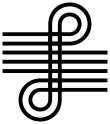
\includegraphics[width=0.15\textwidth]{../Grafiken/Logo_HfM_KA}\par
	
	\vspace{0.6cm}
	
	%Kopfzeile
	{\scshape\LARGE Hochschule für Musik Karlsruhe \par
		\vspace{0.2cm}
		\large Institut für Musikwissenschaft und Musikinformatik\par}
	\vspace{1cm}
	
	%Modul-Angabe
	{\Large \modulname –\modulkuerzel\par}
	
	\vspace{4.5cm}
	
	%Titel
	{\Huge\textbf{\titel}}\par
		{\huge\textsl{\untertitelI\\}}\par
		{\huge\textsl{\untertitelII\\}}
	\vspace{4.5cm}

	%Verfasserangaben
	{Vorgelegt von\par
		\textsc{\verfasser} \par
		\vspace{0.4cm}
		Matrikel-Nr.\matrikelnummer \par
		\adresse \par
		\email \par}
	\vspace{0.3cm}
	
	%Datum
	{\large \abgabedatum}
\end{titlepage}

%To-Do-Liste (Wird bei Option "druckfreigabe" nicht angezeigt)
\ToDoList

\tableofcontents{\protect \thispagestyle{empty}}

\newpage{}
\setcounter{tocdepth}{2}
\pagenumbering{arabic}
\setcounter{page}{1}
\pagestyle{scrheadings}

%Textinhalt des Dokumentes. Beliebig erweiterbar durch weitere Dateien.
% Benutzt mann \include{file} statt \input{file} wird für jeden include eine neue Seite Begonnen, egal wie viel Platz auf der Seite davor ist. Bei \input{file} wird die Seite normal weitergeführt. \include{file} eignet sich besser für Buch-Kapitel, \include{file} mehr für Artikel und Aufsätze.
\begin{spacing}{1,5}

\IfFileExists{HfM-KA-IMWI-HA-Vorwort}{\label{Vorwort}%Vorwort

\mysection{0}{Vorwort}

\textbf{Hier steht das Vorwort zu deiner Arbeit.}

\blindtext
}{}
\newpage
\IfFileExists{HfM-KA-IMWI-HA-Kapitel_01}{\label{Kapitel-01}%Kapitel 1

\section{Das erste Kapitel}

\begin{spacing}{1}
\begin{itemize}
	\item \info{Unterstreicht ein Wort und führt zur Sprechblase am Rand} Notizen zu Kapitel 1
\begin{itemize}
	
\item Hier steht Text\autocite[Vgl.][55\psqq]{Buch1}
\item \enquote{Hier steht noch [...] mehr Text}\autocites(Auslassung: \verfasser)[2]{Buch1}

\end{itemize}
\end{itemize}
\end{spacing}

Da wir Texte lieben und vor allem auch Fußnoten\autocite[1-X]{biblatex1} hier noch eine. 


Hier ist eine weitere\unsicher[fancyline, author=Korrektor]{Hellgrauer Pfeil direkt zu der Stelle, auf die sich die Anmerkung Bezieht} Anmerkung notwendig.

\blindtext

\verbessern{dieser Teil ist noch zu schlecht}Bla bla blaaaa
\newline

Was es hier noch Anzumerken gibt ist die schöne Lösung nicht von Forte oder \textit{piano} sprechen zu müssen, sondern die Standardsymbole \dynmark{f} und \dynmark{p} im Fließtext verwenden zu können.
Das sieht gleich viel professioneller aus, vor allem bei moderneren Angaben wie \dynmark{sfmf}.\info{Dieser Befehl löscht sich nicht automatisch wenn man die Option "print" aktiviert. Daher wird dieser recht obsolete Befehl beim nächsten Update vsl. Entfernt.}\perfekt

\blindtext

\begin{center}
\missingfigure[figwidth=7.2cm]{Hier ist Platz für ein Bild \ldots}
\end{center}

\blindtext

\textsl{Nun noch ein Beispiel für das Blockzitat:}

\begin{Blockzitat}
	\blindtext\autocite{Buch2}
\end{Blockzitat}
}{}
\IfFileExists{HfM-KA-IMWI-HA-Kapitel_02}{\label{Kapitel-02}\input{HfM-KA-IMWI-HA-Kapitel_02}}{}
\IfFileExists{HfM-KA-IMWI-HA-Kapitel_03}{\label{Kapitel-03}\input{HfM-KA-IMWI-HA-Kapitel_03}}{}
\IfFileExists{HfM-KA-IMWI-HA-Kapitel_04}{\label{Kapitel-04}\input{HfM-KA-IMWI-HA-Kapitel_04}}{}
\IfFileExists{HfM-KA-IMWI-HA-Kapitel_05}{\label{Kapitel-05}\input{HfM-KA-IMWI-HA-Kapitel_05}}{}
\IfFileExists{HfM-KA-IMWI-HA-Kapitel_06}{\label{Kapitel-06}\input{HfM-KA-IMWI-HA-Kapitel_06}}{}
\IfFileExists{HfM-KA-IMWI-HA-Kapitel_07}{\label{Kapitel-07}\input{HfM-KA-IMWI-HA-Kapitel_07}}{}
\IfFileExists{HfM-KA-IMWI-HA-Kapitel_08}{\label{Kapitel-08}\input{HfM-KA-IMWI-HA-Kapitel_08}}{}
\IfFileExists{HfM-KA-IMWI-HA-Kapitel_09}{\label{Kapitel-09}\input{HfM-KA-IMWI-HA-Kapitel_09}}{}
\IfFileExists{HfM-KA-IMWI-HA-Kapitel_10}{\label{Kapitel-10}\input{HfM-KA-IMWI-HA-Kapitel_10}}{}
\end{spacing}

\newpage
\section{Literaturverzeichnis}
\label{vz:Literatur}


\printbibliography[heading=none]

%Anhang zum vorliegenden Dokument.
\begin{spacing}{1}
\IfFileExists{HfM-KA-IMWI-HA-Anhang_01.tex}
{\newpage
	\section{Anhang}
	\label{sec:Anhang}
	\label{sec:Anhang-01}
	%Anhang_01

\subsection{Zu den Abbildungen}

Hier gibt es die Möglichkeit selbst Dinge in den Anhang zu schreiben. Beispielsweise eine Tabelle oder Übersicht.
\newline

Standardmäßig ist hier ein Zeilenabstand von 1,0 definiert.
\newline

\blindtext
}{}
\IfFileExists{HfM-KA-IMWI-HA-Anhang_02.tex}
{\newpage
	\label{sec:Anhang-02}
	\input{HfM-KA-IMWI-HA-Anhang_02}}{}
\IfFileExists{HfM-KA-IMWI-HA-Anhang_03.tex}
{\newpage
	\label{sec:Anhang-03}
	\input{HfM-KA-IMWI-HA-Anhang_03}}{}
\IfFileExists{HfM-KA-IMWI-HA-Anhang_04.tex}
{\newpage
	\label{sec:Anhang-04}
	\input{HfM-KA-IMWI-HA-Anhang_04}}{}
\IfFileExists{HfM-KA-IMWI-HA-Anhang_05.tex}
{\newpage
	\label{sec:Anhang-05}
	\input{HfM-KA-IMWI-HA-Anhang_05}}{}
\end{spacing}

\IfFileExists{../PDF-Anhaenge/HfM-KA-IMWI-HA-PDF-Anhang_01.pdf}
{\label{sec:Anhang-PDF-01}\include{HfM-KA-IMWI-HA-PDF-Anhang_01.pdf}}{}
\IfFileExists{../PDF-Anhaenge/HfM-KA-IMWI-HA-PDF-Anhang_02.pdf}
{\label{sec:Anhang-PDF-02}\include{HfM-KA-IMWI-HA-PDF-Anhang_02.pdf}}{}
\IfFileExists{../PDF-Anhaenge/HfM-KA-IMWI-HA-PDF-Anhang_03.pdf}
{\label{sec:Anhang-PDF-03}\include{HfM-KA-IMWI-HA-PDF-Anhang_03.pdf}}{}
\IfFileExists{../PDF-Anhaenge/HfM-KA-IMWI-HA-PDF-Anhang_04.pdf}
{\label{sec:Anhang-PDF-04}\include{HfM-KA-IMWI-HA-PDF-Anhang_04.pdf}}{}
\IfFileExists{../PDF-Anhaenge/HfM-KA-IMWI-HA-PDF-Anhang_05.pdf}
{\label{sec:Anhang-PDF-05}\include{HfM-KA-IMWI-HA-PDF-Anhang-05.pdf}}{}

\thispagestyle{plain}
\section{Selbstständigkeitserklärung}
\vspace{0,4cm}

\framebox{
	\parbox[c]%Position
	[0.2\textheight]%Höhe
	[l]%Textposition
	{\textwidth}%Breite
	{Mit meiner Unterschrift bestätige ich, dass ich das hier vorgestellte Praktikum absolviert und diesen Bericht selbstständig verfasst habe.\\
		\\ \\ \\ 
		
		\begin{tabular}{lp{2em}l} 
			Karlsruhe, den \abgabedatum & &\\
			\cline{1-1}\cline{3-3}  Ort, Datum\hspace{3cm} & \hspace{3cm} & \verfasser \hspace{3cm}
		\end{tabular}}
	}

\end{document}